%!TEX root = ../../../exa-ma-d7.1.tex
%\chapter{Work Package 1: Discretization}
%\label{chap:wp1}

\section{Objectives \& Context}
% • Which Exa-MA bottlenecks (B#) WP1 addresses  
% • Relation to overall strategy (high-order methods, meshing, adaptivity)  
% • List of key tasks T1.1–T1.7
This work package deals with two main points: 
\begin{itemize} 
\item {\bf Geometric domain representations and their discrete counterparts (such as meshes)}. \\
Computation domain representation is usually the main starting point and support of the simulation. WP1 works on challenges related to geometric representation robust to defects and resilient to heterogeneous input, but also on mesh adaptivity and efficient parallel representations of large-scale models.\\
This point is related to the bottlenecks [B2, B6, B7, B9, B11-B13]. 
\item {\bf Physics-based models.}\\
These models need to include multiple phenomena or process couplings at multiple
scales in space and time. Space and time adaptivity are then mandatory. Time integration requires special care to become more parallel, more asynchronous, and more accurate for long-time simulations. In WP1, we focus on (a) high-order methods to increase the
computational intensity and reduce communications and (b) nonconforming or partitionned methods that are
designed to avoid/reduce/minimize communications.\\
This point is related to the bottlenecks [B7, B10].
\end{itemize}

This work package is ambitious and hence includes many tasks and subtasks. \textcolor{red}{from IR : on peut citer le document scientifique ici??} The thematic of the main tasks are recalled hereafter.
\begin{itemize}
    \item {\bf T1.1: Mesh generation}\\
    This task embeds valid large-scale generation, mesh generation for non-conforming methods and all-hexahedral block grids.
%    {\bf T1.1.1 Valid large-scale mesh generation.} We will explore the automated generation of large-scale meshes, either from measurement data or from designed CAD models. Such input data require 3D reconstruction and meshing algorithms capable of dealing with heterogeneous, defect-laden representations. We will look for meshing algorithms that scale, and are unconditionally robust to input defects. Valid meshing herein translates into output meshes that are watertight and without self-intersections. The meshing algorithms will also provide detail levels with fine-grain and adjustable balance between complexity, resolution and approximation.\\
%{\bf T1.1.2 Mesh generation for non-conforming methods.} In the framework of non-conforming domain decomposition, two-level mesh generation algorithms will be explored and implemented. The macro elements are independently refined, in parallel, into fine meshes with no conformity requirement along the boundaries of the macro elements. The coarse grid must support partitioning and dynamic load balancing when proceeding to fine mesh adaptation. Mesh connectivity must be available and shared efficiently between neighboring macro-elements.\\
%{\bf T1.1.3 Mesh generation of all-hexahedral block grids.} In this task, we develop robust hexahedral block structured meshes, based on state-of-the-art algorithms and open-source software to derive linear block structure that will be a support to: (1) Curve them to yield high-order blocks, and (2) Define local grid patterns that fit the multigrid method requirements and can be applied in each block or even onto several connected blocks.\\
    \item {\bf T1.2 Adaptive Mesh Refinement for unstructured grids.} 
%  Mmg/ParMmg is a framework that can adapt to very large meshes, currently up to several billion cells. ParMmg is a MPI-based component for parallel mesh adaptation. Our objective is to break new scalability barriers in Mmg/ParMmg through (i) code robustification, (ii) improved memory management, (iii) graph coloring and interface migration with load balancing, (iv) metrics management, (v) benchmark, profile and optimization.
    \item {\bf T1.3 Adaptive Mesh Refinement for Cartesian or block grids.}
%We use Adaptive Mesh Refinement (AMR) methods to improve accuracy and computation time in simulations, particularly when dealing with spatially localized physical phenomena. Several strategies for error control are presented, including patch-based, cell-based and adaptive multiresolution using wavelets. Large-scale simulations using AMR typically rely on specialized data-structures. We focus on several discretization methods (finite elements, finite volumes, and finite differences), conforming or non-conforming, with structured mesh refinement using all-hexahedral/quadrilateral elements for exascale simulations. We also propose to work on HPC algorithm extensions of the local multigrid AMR methods to develop load-balancing algorithms and efficient refinement strategies.
    \item {\bf T1.4 Finite Element Exascale Framework}
%    We utilize exascale hardware and low-level software infrastructure to create a framework for high-order/spectral finite element methods on unstructured grids. We aim at providing a framework that can handle the full de Rahm complex, while hiding low-level architecture details. The focus is on non-conforming methods to provide optimized kernels for finite elements, which will require close collaboration with PC2’s WP2 and WP3.
    \item {\bf T1.5 Exploit non conforming methods for efficient parallel parallel}
    
%   Conformal finite-element discretizations lead to large sparse linear systems that are difficult to solve with modern parallel architectures. We propose to explore non-conformal methods such as Trefftz methods, hybridizable discontinuous Galerkin (HDG) methods, including HHO and the mortar element method, as alternatives to cG. We aim at improving the conditioning of the resulting system for efficient iterative solution procedure or reducing the size of the sparse linear system to be solved. Our plan is also to work on thecombination of these methods and domain decomposition methods in order to accelerate theconvergence of iterative solvers.
    \item {\bf T1.6 Time-strategy for evolution equations when the mesh is dynamically adapted}\\
    This tasks embeds parallel in time strategies and error control in time.
%{\bf T1.6.1 Parallel in time strategies: improve coarse solver.} The time-parallelization methods, such as the parareal method, propose to use domain decomposition techniques in the time direction to solve more rapidly on distributed architectures. However, there are still issues to be addressed to improve efficiency, such as the efficiency of the coarse solve, the coupling of different PDEs with at least a parabolic PDE and the extension to Hamiltonian systems.
% {\bf T1.6.2 Error control in time.} We consider the challenges of solving evolving multiscale problems. Two types of multiscale problems are mentioned: those with relaxation sources and short time scales, and those with complex sources involving a broad spectrum of scales. The first type can lead to inefficient use of mesh adaptation and strong stability constraints must be met. Two key issues are addressed: designing numerical schemes with strong stability properties and preserving invariant convex spaces. For the second situation, some schemes based on adaptive operator splitting and adaptive multiresolution have been developed. Three breakthroughs are needed to tackle exascale simulations: quantifying compression errors, extending to high order methods and wavelets, and designing new time integration strategies.
    \item {\bf T1.7 Efficient multimodel/multiphysics coupling}\\
    This tasks embed multiphysics partitioned discretization and multiscale coupling.    
%{\bf T1.7.1 Multiphysics partitioned discretization.} We need far more realistic simulations of multiphysics problems and the importance of scalability in these simulations. Our focus is on partitioned coupling, using well-established discretization methods for each physics that have demonstrated good scalability properties. The task involves studying scalable coupling algorithms and ensuring that the properties of the system obtained after discretization meet the scaling requirements, with a focus on fields’ projections and conservations. This task is related to task T3.5 of WP3 on exascale simulations of partitioned multiphysics coupling. We will also consider adaptive high order coupling techniques to take advantage of partitioning for high performance computing without compromising on accuracy of the system, even when dealing with DAEs and elliptic/parabolic equations.
% {\bf T1.7.2 Multiscale coupling} Numerical methods, such as discontinuous Galerkin discretizations, are conducive for exascale computing because they allow for non-conformal discretization. These methods can rely on a primal formulation set on the skeleton of a coarse mesh and a dual one involving the solution of small problems solved at the element level. The use of different basis functions and numerical methods, such as those based on multiscale finite elements or neural networks, can be used to reproduce different physics.
%
\end{itemize} 

\section{Scientific Advances}

\subsection{Task 1.1 - Mesh generation}
The advances in this task concern valid large-scale generation and especially feature-preserving alpha wrapping.

The Alpha Wrapping algorithm implemented in the CGAL library provides a robust method for generating a watertight, orientable, and manifold surface mesh that conservatively encloses a 3D input. It is particularly effective when the input is noisy, incomplete, or non-manifold. The algorithm proceeds as follows:

\begin{enumerate}
\item Delaunay Triangulation: A 3D Delaunay triangulation is constructed from the input geometry, which may consist of point clouds, triangle soups, or polygon soups.
\item Shrink-Wrapping via Gate Propagation: A priority queue of triangle facets (termed gates) is used to traverse the triangulation from the exterior inward, simulating a wrapping process.
\item Steiner Point Insertion and Offset Projection: Inner structures and defects are filtered by inserting Steiner points and projecting circumcenters onto a user-defined offset surface.
\item Surface Extraction: A final surface mesh is extracted from the triangulation, enclosing the input within the prescribed offset.
\end{enumerate}

The resulting mesh is guaranteed to be watertight, orientable, and 2-manifold, even in the presence of severe input corruption.

Strengths
\begin{itemize}
\item Robustness: Handles raw, noisy, and non-manifold input gracefully.
\item Conservative enclosure: Guarantees that the output mesh strictly contains the input geometry.
\item Flexibility: Works with triangle soups, polygon soups, and point clouds.
\item Parameter control: Users can tune two parameters (alpha and offset) to balance tightness vs. mesh simplicity.
\item Guaranteed termination: Always produces a valid output mesh.
\end{itemize}

Limitations
\begin{itemize}
\item Loss of geometric detail: Fine-scale features, cavities, and internal structures are typically smoothed out.
\item No Sharp Feature Preservation: The method does not retain sharp edges or creases. Its reliance on Delaunay triangulation and circumradius-based traversal inherently favors smooth, rounded surfaces. Without explicit feature detection or edge-aware refinement, sharp creases are interpreted as noise and are systematically smoothed during wrapping.
\item Mesh complexity trade-off: Achieving tighter wraps may require additional Steiner points, increasing computational cost and mesh density.
\end{itemize}

These limitations make the standard Alpha Wrapping algorithm unsuitable for applications such as reverse engineering or CAD, where sharp features are critical. To address this, we investigated a feature-preserving variant of the algorithm.

\paragraph{Feature-Preserving Variant: Salient Steiner Points.}

Our approach modifies the definition of Steiner points computed on-the-fly during wrapping, which combines Delaunay refinement with geometric carving. In the original method, Steiner points are derived either from intersections between Voronoi edges and the offset surface, or from projections of Voronoi vertices onto the offset surface. We propose instead to compute Steiner points that correspond to salient feature locations.

Here, features encompass not only corners and creases, but also less conventional singularities such as cusps, darts, tips, and non-manifold configurations. Detecting such features is inherently ill-posed, and no universal definition of saliency exists. Intuitively, saliency denotes the geometric or perceptual prominence of a feature (typically a crease or corner) relative to its local surface context.

Common approaches estimate saliency via scalar fields that capture local contrast in curvature, dihedral angle, or normal variation. While effective in post-processing, these methods are insufficient for our purposes, as we aim to detect sharp features during the wrapping process. In particular, the local configuration of the evolving wrap must be taken into account. Multi-scale analysis can identify persistent features across resolutions, but it does not incorporate the dynamic context of wrapping.

\paragraph{Visibility-Based Criterion for Salient Point Selection}

A further challenge lies in selecting Steiner points that facilitate subsequent mesh refinement, with the goal of minimizing final mesh complexity and optimizing the complexity–distortion trade-off. After extensive experimentation, we developed a promising criterion based on 3D visibility, tailored to the local wrapping context.

For a candidate Steiner point on the offset surface, we compute a weighted sum of two visibility volumes: (1) The volume visible from the point to the current wrap, and (2) The volume visible from the point to the offset surface itself.

% 2D figure ?

A higher weight is assigned to visibility toward the wrap, reflecting its role in guiding the wrapping frontier. Formally, the visible volume from a point $p$ in a 3D domain $\Omega$ is defined as the set of all points $q \in \Omega$ such that the line segment $\overline{pq}$ lies entirely within $\Omega$, unobstructed by any surface or obstacle.

Computing these volumes is non-trivial due to two factors: (1) Aware Visibility: Even though the wrap is represented as a surface triangle mesh, obstacles necessitate splitting empty tetrahedra (formed by connecting the candidate point to wrap triangles) into smaller tetrahedra to accurately model occlusion, and (2) Offset Geometry: The offset surface is only implicitly defined as the locus of points at a fixed distance from the input, and is piecewise curved, complicating visibility estimation as requiring a cubature or approximations.

Such a visibility-based criterion offers a principled way to select Steiner points that are both geometrically meaningful and computationally advantageous, paving the way for feature-aware alpha wrapping.

\subsection{Task 1.5 - Exploit non conforming methods for efficient parallel parallel}
A hybridizable discontinuous Galerkin (HDG) method has been developed to solve the linear anisotropic elastic equation in the frequency domain. HDG discretization allows us to decrease the size of the discrete system while keeping a good conditioning of the global matrix to be inverted. First-order formulation with the compliance tensor and Voigt notation are employed to provide a compact description of the discretized problem and flexibility with highly heterogeneous media. We further focus on the question of optimal choices of stabilization in the definition of HDG numerical traces. For this purpose, we construct a hybridized Godunov-upwind flux for anisotropic elastic media possessing three distinct wavespeeds. This stabilization removes the need to choose a scaling factor, contrary to the identity and Kelvin–Christoffel based stabilizations which are popular choices in the literature. We carry out comparisons among these families for isotropic and anisotropic material, with constant background and highly heterogeneous ones, in two and three dimensions. These experiments establish the optimality of the Godunov stabilization which can be used as a reference choice for a generic material in which different types of waves propagate. This work has been presented in conferences (Eccomas, Waves2025) and is published \cite{pham_numerical_2024}.

\subsection{Task 1.7 -  Efficient multimodel/multiphysics coupling}
We have launched a work on efficient multiphysics partitioned strategies in the HPC framework. Our approach is intended to be as generic as possible and to consider black-box physical solvers. The application of interest will be elasto-acoustic and thermal-elastic problems.\\
This work is carried out since November 2024 by Pierre Dubois, PhD student, managed by the CEA team (Isabelle Ramière, Raphaël Prat) and the Inria Makutu project team (Hélène Barucq).

A review of the literature on numerical methods for multiphysics couplings has been done. Moreover, a review of existing multiphysics HPC strategies has also been carried out. The partitioned coupling seems promising as it enables reusing efficient standalone HPC solvers. The use of an acceleration fixed-point strategy may be required to enable convergence.

The quasi-static problem setting has been adopted for both elasto-acoustic and thermal-elastic couplings. A thermal-elastic strong coupling benchmark has been selected and tested on the sequential finite element solver Cast3M. The porting to the HPC MFEM library is ongoing work.



\section{Application Showcase}

% %!TEX root = ../../../../exa-ma-d7.1.tex

\section{Demonstrator: Elliptic linear PDE: CG}

We present here the demonstrator to numerically solve elliptic linear PDE using continuous Galerkin approach.
Precisely, we solve here the heat transfer equation.

\Cref{tab:app-feelpp-discr-1} describes the specifications of the application.

\begin{table}[ht]
    \centering
    \begin{tblr}{
        colspec = {l X[10cm]},
        row{odd} = {numpexlightergray},
        hlines = {0.1pt, numpexgray},
        vlines = {numpexgray},
        row{1} = {numpexgray, fg=white, font=\bfseries},
    }
        Field & Details \\
        id & \texttt{app-feelpp-discr-1} \\
        name & Discretization \\
        Partners & Unistra \\
        PC & PC1 - ExaMA, PC2 - ExaSoft \\
        Responsible (Permanent) & V. Chabannes; C. Prud'homme \\
        WP7 Engineer & Thomas Saigre (UNISTRA) \\
        work\_package & WP1, WP3 \\
        application\_type & extended-mini-app \\
        purpose &  Solve a PDE (heat, solid mech) with different discretization methods from low to high order \\
        Method-Algorithm WP1 & unstructured mesh, finite element, dG/hdG, cG, spectral element \\
        Method-Algorithm WP2 & \\
        Method-Algorithm WP3 & domain decomposition methods, Krylov solver, preconditioning \\
        Method-Algorithm WP4 & \\
        Method-Algorithm WP5 & \\
        Method-Algorithm WP6 & \\
        WP7 & \\
        outputs & Gmsh, JSON config	JSON small-data, JSON reports, in-house, Markdown or Asciidoc \\
        metrics & \texttt{benchmark-verification}, \texttt{strong-scalability}, \texttt{weak-scalability}, \texttt{io-scaling} \\
        status & benchmark-ready \\
        Benchmark scope & full-system, method-verification, solver-scaling \\
        Framework & Feel++, PETSc \\
        parallel\_framework & MPI, Kokkos \\
        spec\_due & 6/15/2025 \\
        proto\_due & 7/1/2025 \\
        repo\_url & \url{https://github.com/numpex/apps-feelpp}\\
    \end{tblr}
    \caption{Description of the demonstrator \texttt{app-feelpp-discr-1}.}
    \label{tab:app-feelpp-discr-1}
\end{table}



\subsection{Description of the benchmark}


The benchmark known as \emph{thermal bridges} is an example of an application that enables us to validate numerical simulation tools using \Feelpp.
We have developed tests based on the ISO 10211:2017 standard \cite{noauthor_iso_2017}, which provides methodologies for evaluating thermal bridges in building construction.

Thermal bridges are areas within a building envelope where heat flow is different compared to adjacent areas, often resulting in increased heat loss or unwanted condensation.
The standard is intended to ensure that thermal bridges' simulation are accurately computed.
It provides reference values and tolerance on heat temperature and heat flux at several locations of the geometry.

At the mathematical level, this application requires finding the numerical
solution of an elliptic linear PDE, namely the heat equation.
We employ a finite element method based on continuous Lagrange Finite Element of order 1,2 and 3 (denoted by $\mathP_1$, $\mathP_2$, $\mathP_3$),
and we analyze the execution time of the main components of the simulation.

\Cref{fig:spec:app-feelpp-discr-1:thermal_bridges:geometry} represents the geometry
of this benchmark and the domain decomposition by material.% the 3D temperature field solution, and an example of mesh partitioning.

\begin{figure}[!ht]
  \centering
  \begin{subfigure}[c]{0.49\textwidth}
    \centering
    \begin{tikzpicture}
        \draw (0, 0) node {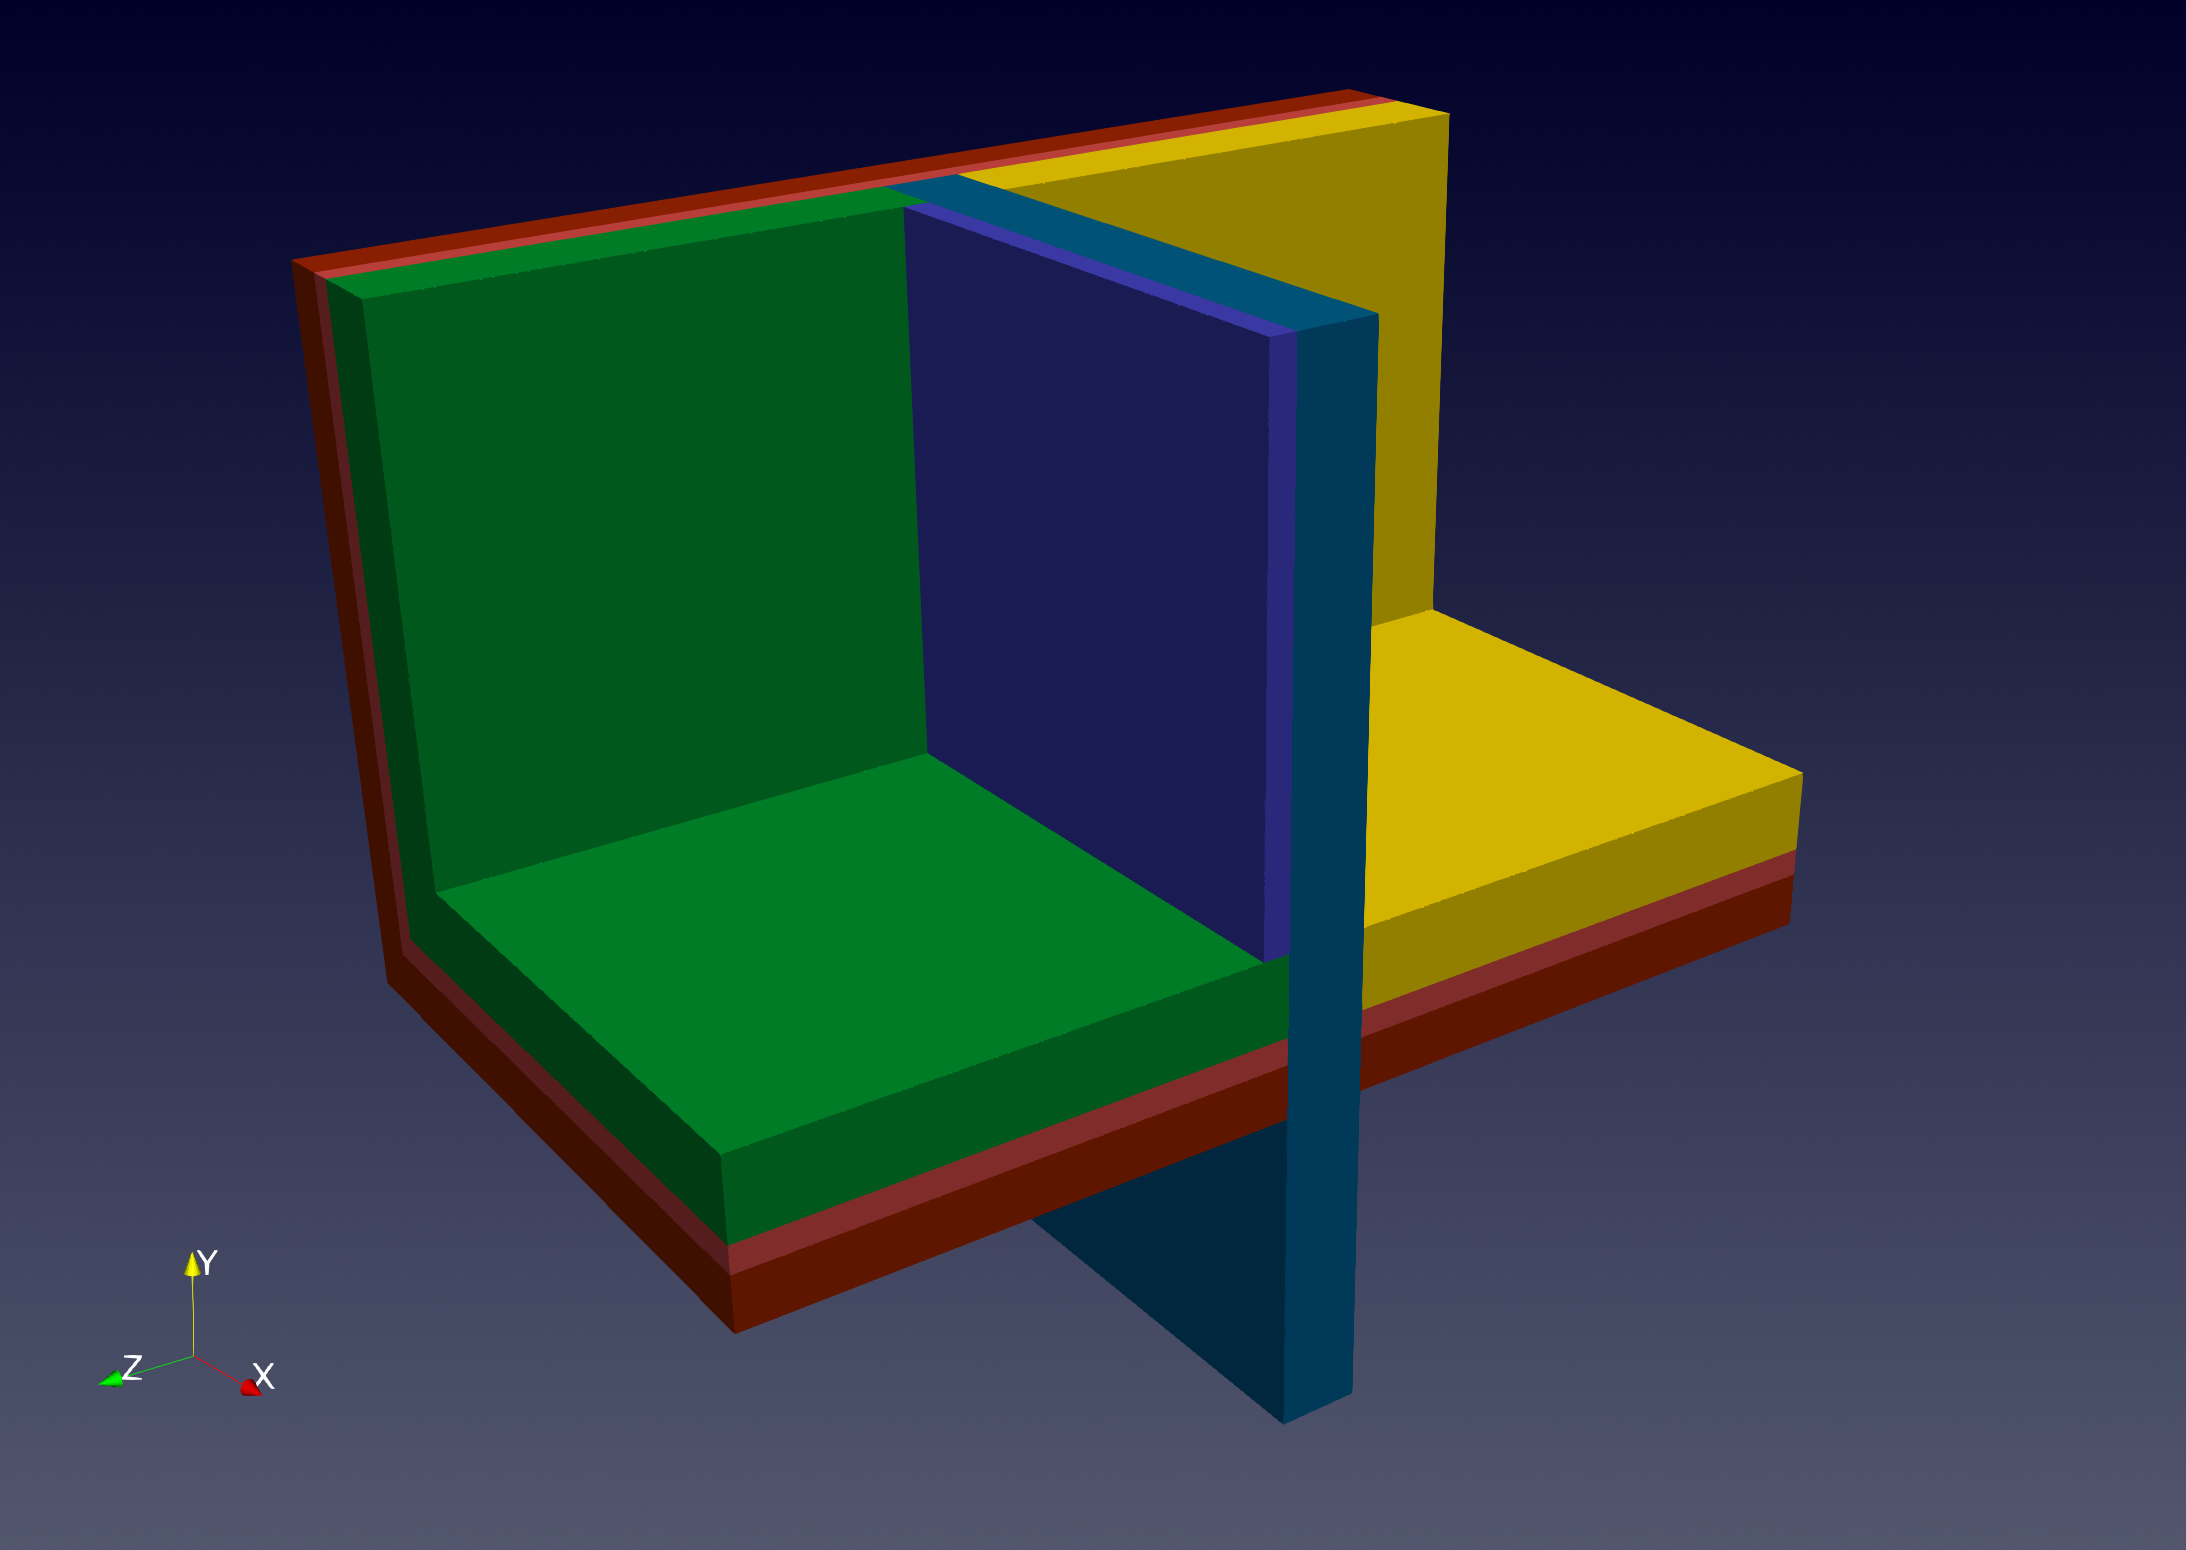
\includegraphics[width=\textwidth]{graphics/feelpp/feelpp-benchmark-thermalbridges-geom.png}};
        \begin{scope}[shift={(2.8, -2.8)}, scale=1.5]
            \draw[red!90!black, ->] (0, 0) -- (0.19, -0.22) node[anchor=west] {$x$};
            \draw[green!70!black, ->] (0, 0) -- (0, 0.4) node[anchor=west] {$y$};
            \draw[blue!80!black, ->] (0, 0) -- (-0.43, -0.07) node[anchor=south] {$z$};
        \end{scope}
    \end{tikzpicture}

  \end{subfigure}
  \hfill
  \begin{subfigure}[c]{0.49\textwidth}
    \centering
        \begin{tikzpicture}
        \draw (0, 0) node {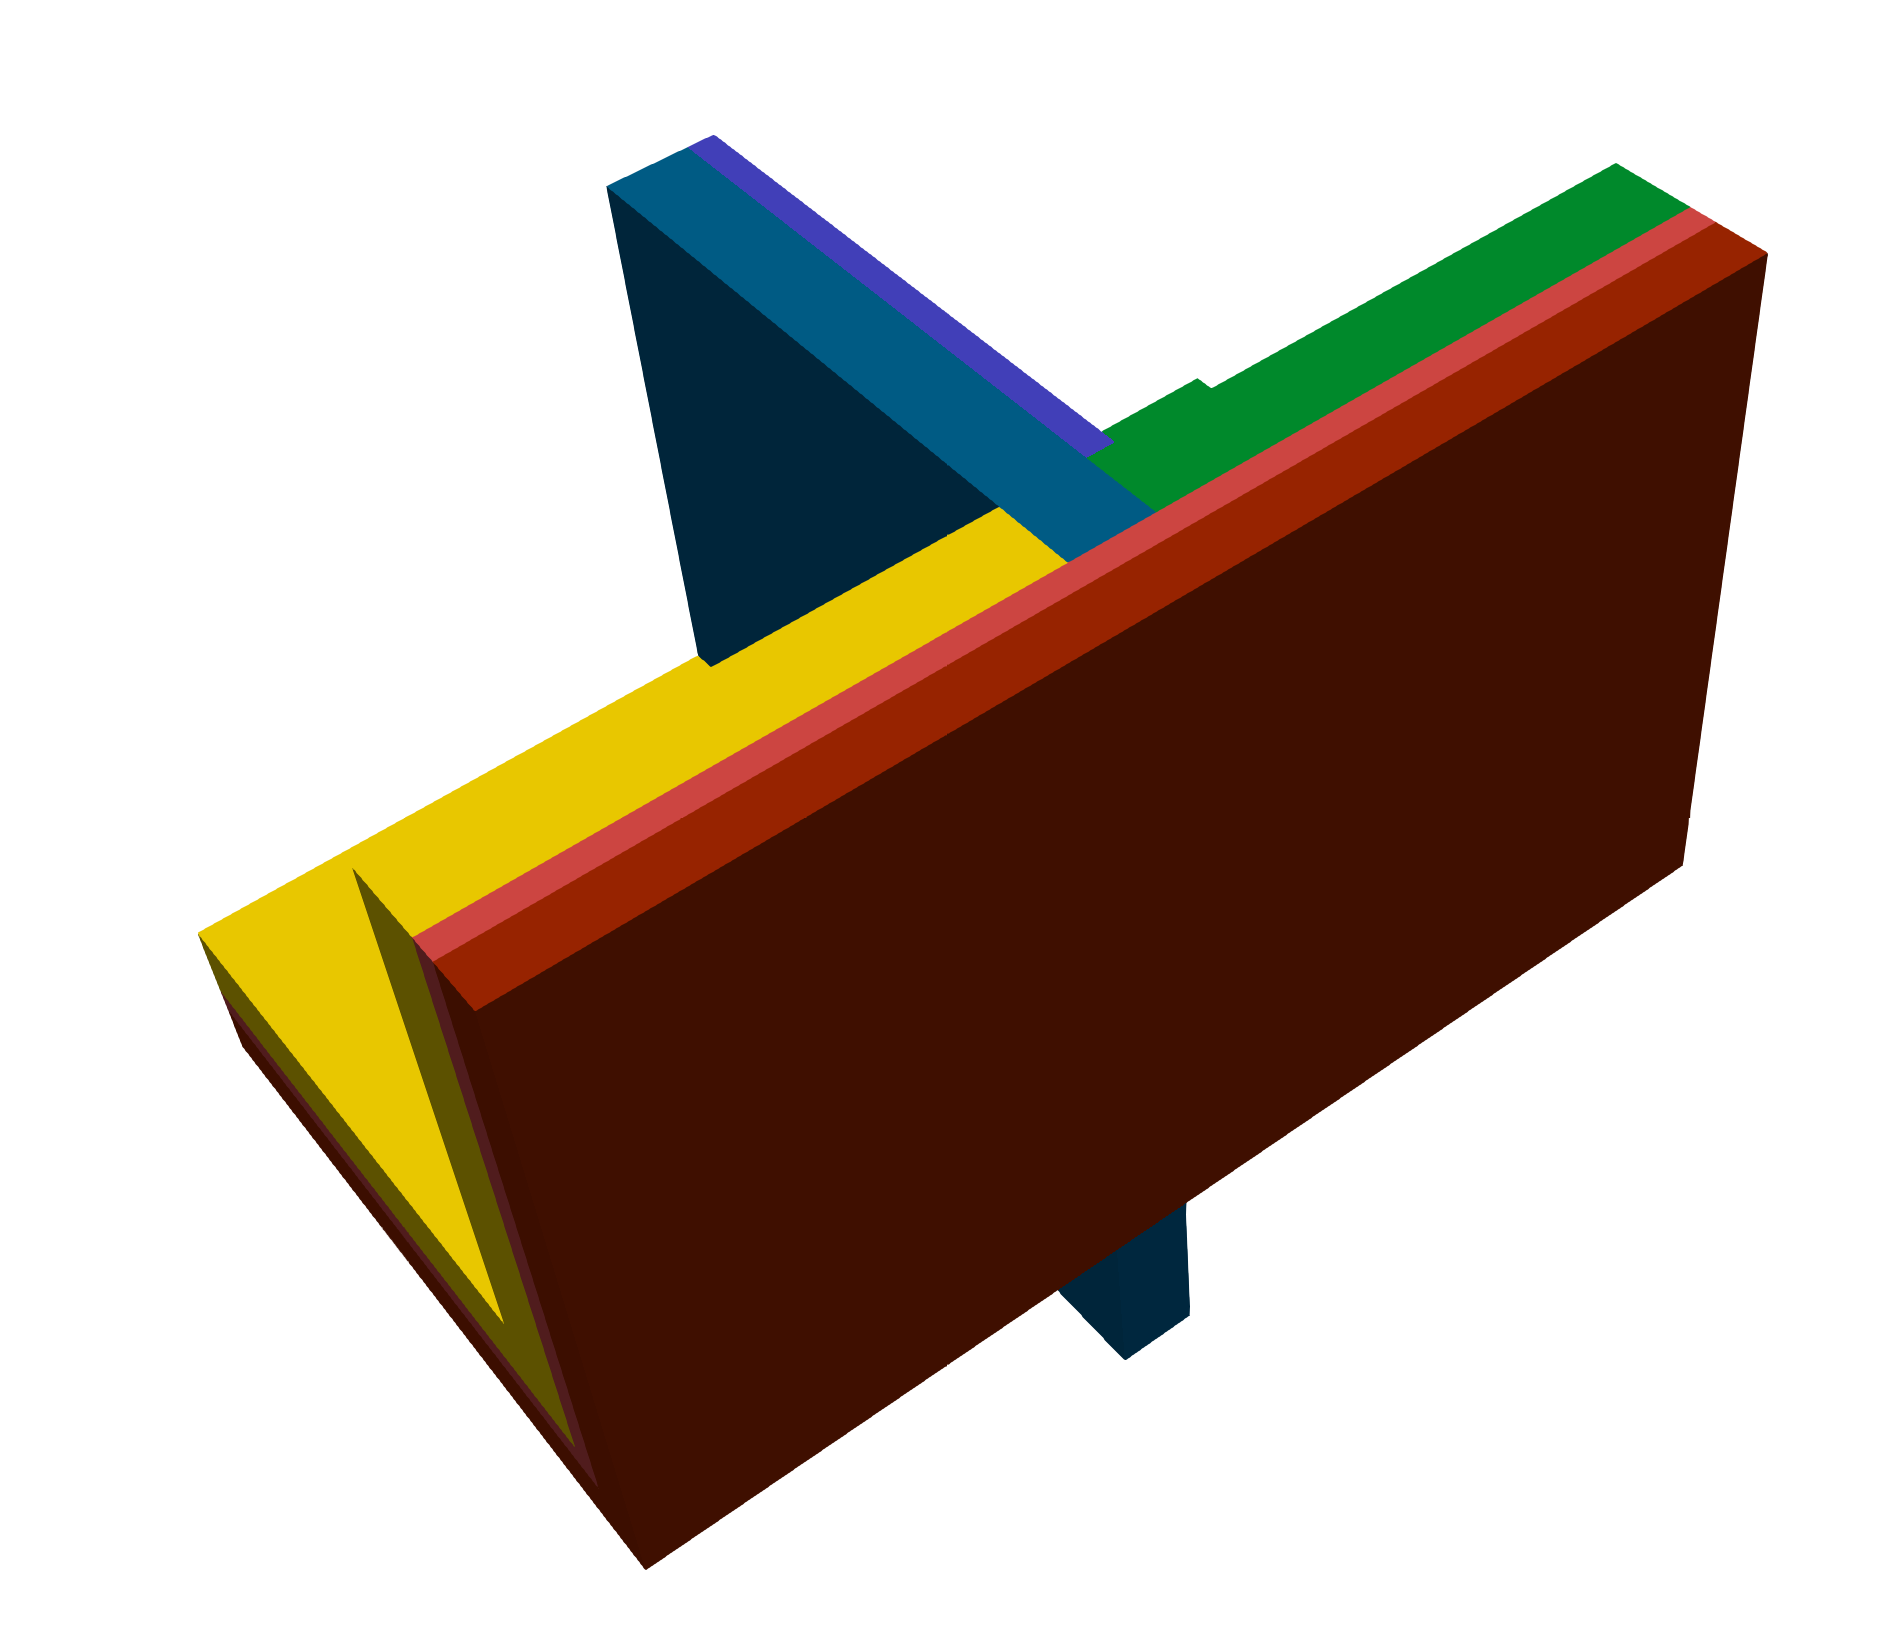
\includegraphics[width=\textwidth]{graphics/feelpp/feelpp-benchmark-thermalbridges-geom2.png}};
        \begin{scope}[shift={(2.8, -2.8)}, scale=1.5]
            \draw[red!90!black, ->] (0, 0) -- (-0.24, 0.22) node[anchor=east] {$x$};
            \draw[green!70!black, ->] (0, 0) -- (-0.04, 0.34) node[anchor=west] {$y$};
            \draw[blue!80!black, ->] (0, 0) -- (0.34, 0.2) node[anchor=north] {$z$};
        \end{scope}
    \end{tikzpicture}
  \end{subfigure}
  \caption{Thermal bridges benchmarks - geometry and materials.}
  \label{fig:spec:app-feelpp-discr-1:thermal_bridges:geometry}
\end{figure}





\subsection{Benchmarking tools used}


The performance tools integrated into the \Feelpp-toolboxes framework were used to measure the execution time.

The metrics measured are the execution time of the main components of the simulation.
We enumerate these parts in the following:
\begin{enumerate}
\item \textbf{Init:} load mesh from filesystem and initialize heat toolbox (finite element context and algebraic data structure).
\item \textbf{Assembly:} calculate and assemble the matrix and right-hand side values obtained using the finite element method.
\item \textbf{Solve:} the linear system by using a preconditioned GMRES.
\item \textbf{PostProcess:} compute validation measures (temperature at points and heat flux) and export on the filesystem a visualization format (EnSight Gold) of the solution.
\end{enumerate}




\subsection{Input/Output Dataset Description}


\subsubsection{Input Data:}
  \begin{itemize}
  \item Meshes: We have generated three levels of mesh called \texttt{M1}, \texttt{M2}
    and \texttt{M3}. These meshes are stored in GMSH format. The statistics can be found in \Cref{tab:spec:app-feelpp-discr-1:thermal_bridges:discr_stat}. We have also prepared for
    each mesh level a collection of partitioned mesh.
    The format used is an in-house mesh format of \Feelpp based on
    JSON+HDF5 file type.
    The GMSH meshes and the partitioned meshes can be found on our Girder
    database management, in the \Feelpp collections.
  \item Setup: Use standard setup of \Feelpp toolboxes. It corresponds to a cfg
    file and JSON file. These config files are present in the GitHub of \Feelpp.
  \item Sif image: feelpp:v0.111.0-preview.10-noble-sif  (stored in the GitHub registry of \Feelpp)
  \end{itemize}

\subsubsection{Output Data:}

The output includes the computed values of validation measure in CSV files format, export visualization files (mesh, partitioning, temperature), and the time taken to perform each simulation step.
Metric:
\begin{itemize}
    \item \texttt{benchmark-verification},
    \item \texttt{strong-scalability},
    \item \texttt{weak-scalability},
    \item \texttt{io-scaling}: time taken by the application to read meshes, and to write the solution on disk (especially reading).
\end{itemize}


\SetTblrInner{rowsep=0pt}
\begin{table}[!ht]
    \centering
    \begin{tblr}{
        colspec={c*{7}{Q[c, cmd=\pgfmathprintnumber]}},
        vlines={numpexgray},
        hlines={numpexgray},
        row{1,2}={bg=numpexgray, fg=white, font=\bfseries, halign=c, cmd=\normalfont},
        rowhead=2, % This option excludes the first two rows from the column command
    }
    \SetCell[c=5]{c}{Mesh properties} & & & & & \SetCell[c=3]{c}{Number of degrees of freedom} & &\\
        Tag & \# points & \# edge & \# faces & \# elements & $\mathP_1$ & $\mathP_2$ & $\mathP_3$ \\
        \texttt{M1} & 193654 & 1299920 & 2164759 & 1058492 & 193654 & 1493574 & 4958253\\
        \texttt{M2} & 1401135 & 9778744 & 16566803 & 8189193 & 1401135 & 11179879 & 37525426\\
        \texttt{M3} & 10572256 & 75307308 & 128722252 & 63987199 & 10572256 & 85879564 & 289909124\\
    \end{tblr}

  \caption{Thermal bridges benchmarks - Statistics on meshes and number of degrees of freedom with respect to finite element approximation}
  \label{tab:spec:app-feelpp-discr-1:thermal_bridges:discr_stat}
\end{table}



%%%%%%%%%%%%%%%%%%%%%%%%%%%%%%%%%%%%%%%%%%%%%%%%%%%%%%%%%%%%%%%%%%%%%%%%%%%%%%%%%%%%%%%%%%%%%%%%%%%%%%%%%%%%%%%%%%%%%%%%

\subsection{Results summary}

\todo{The results here are the one taken from the previous version of D7.1, they will be run again for v2.}


\subsubsection{Numerical solution}

\todo{Insert numerical solution obtained from the toolbox, and the partitioning of the mesh}


\begin{figure}[!ht]
  \centering
  \begin{subfigure}[c]{0.49\textwidth}
    \centering
    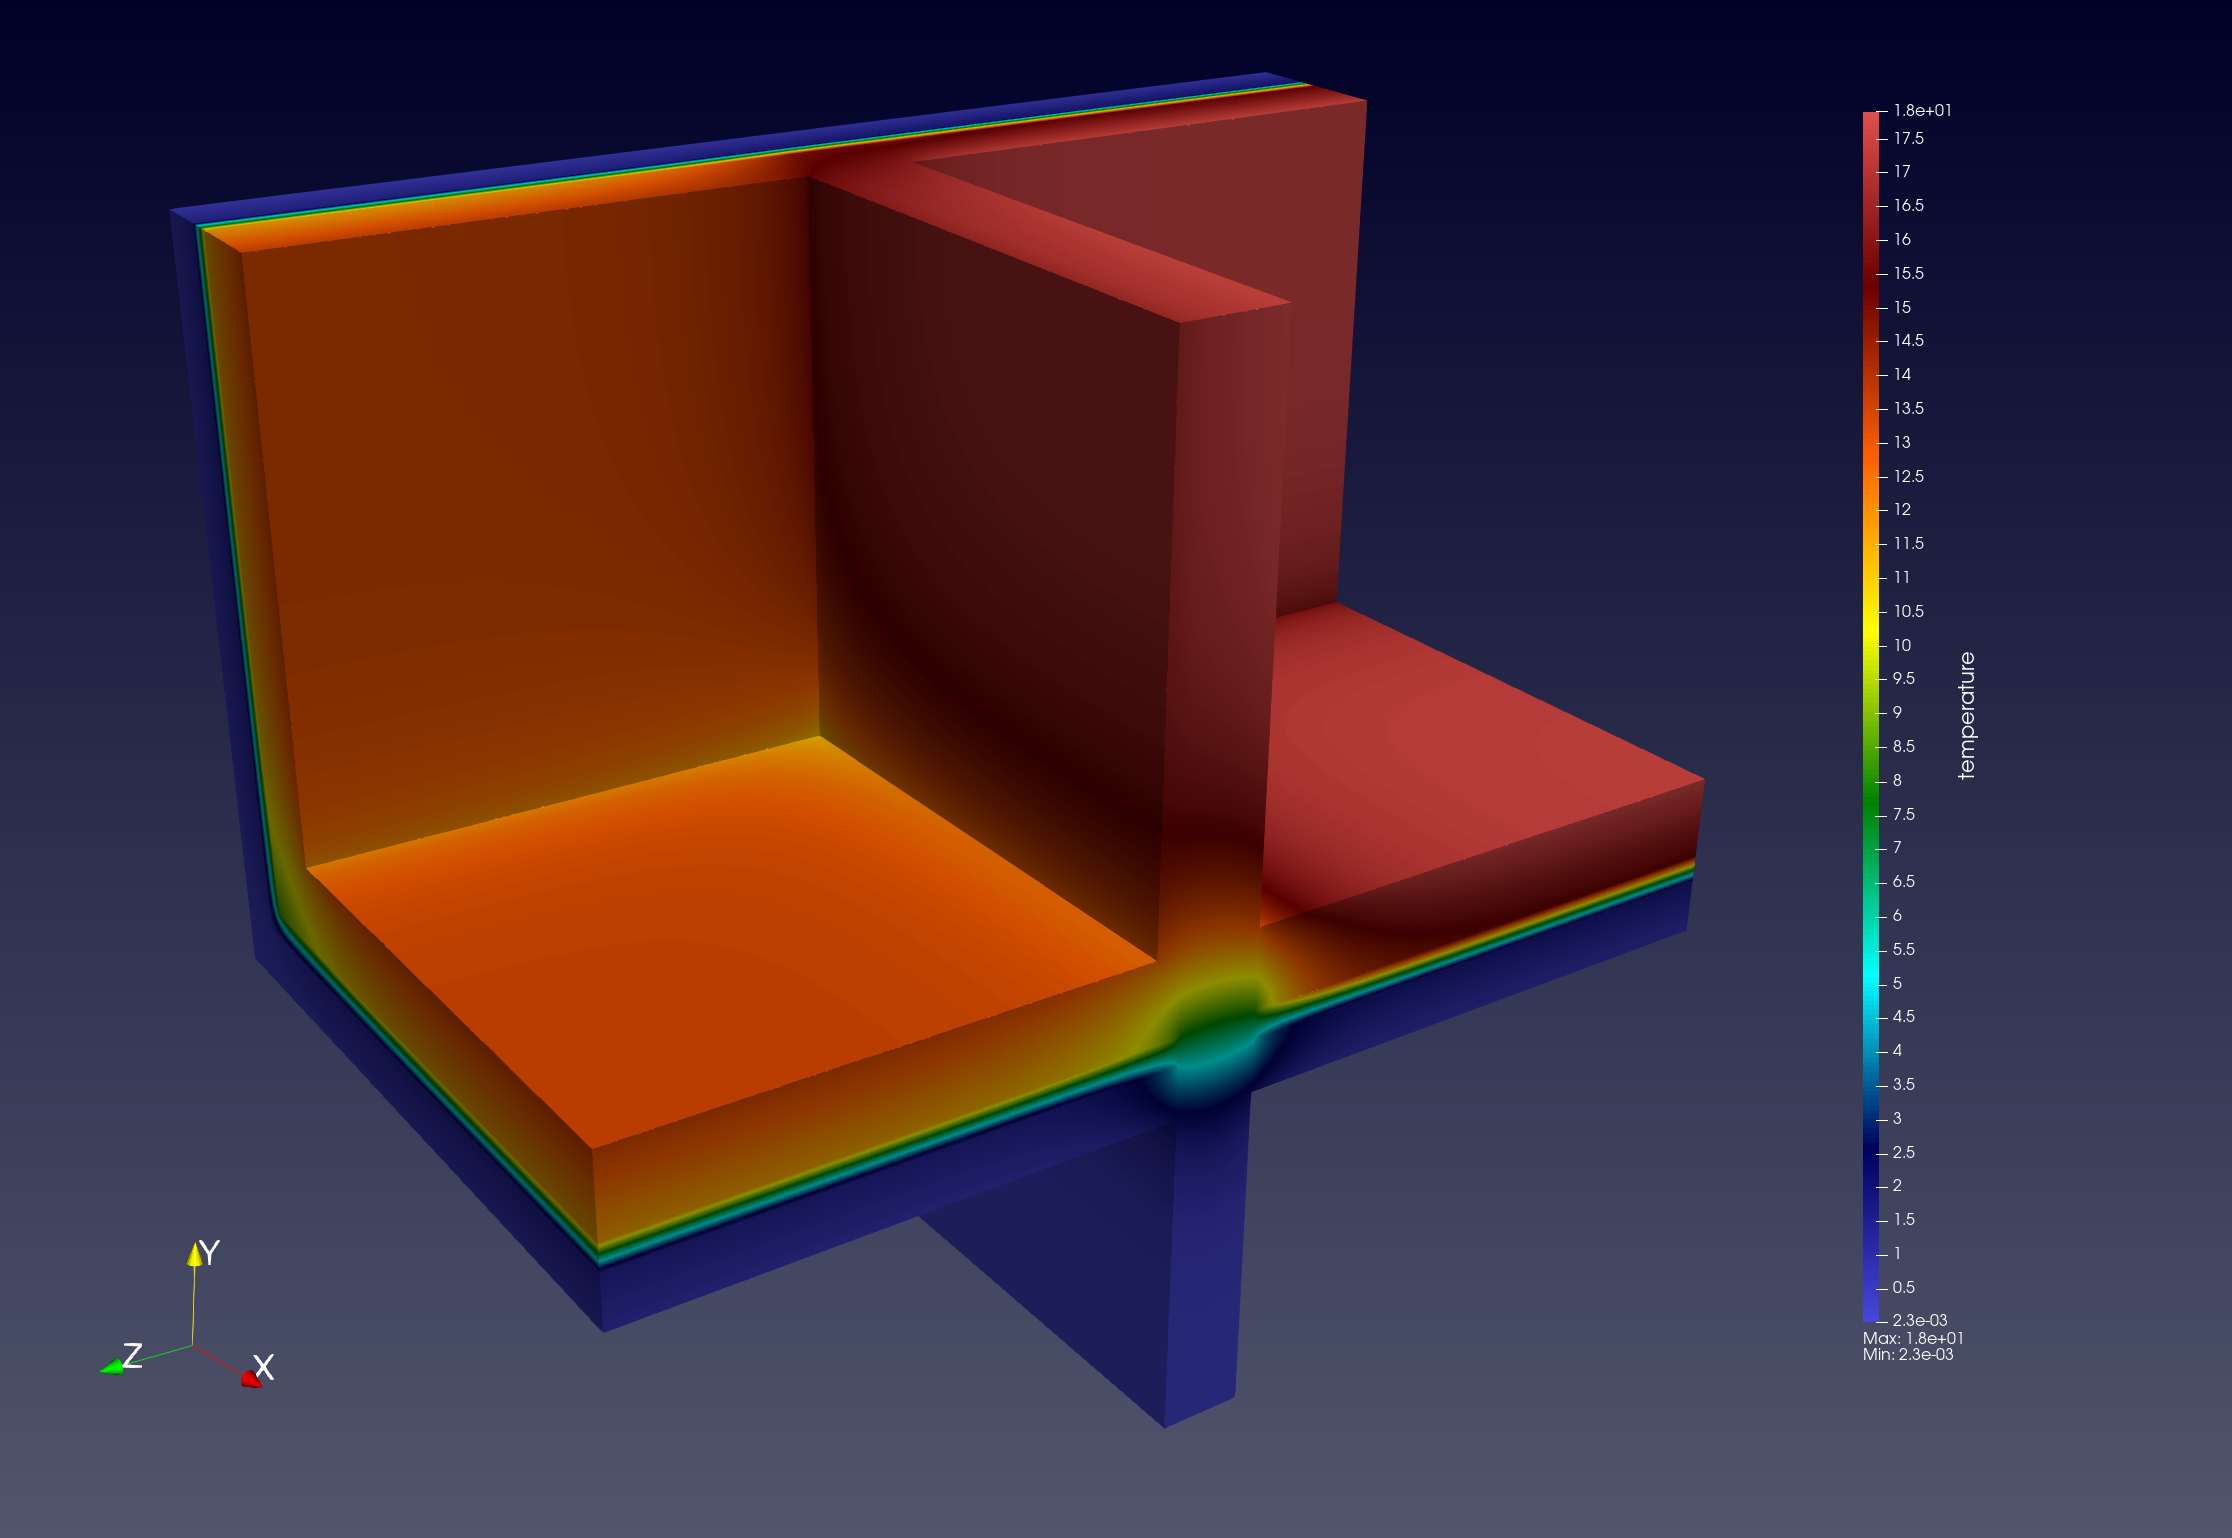
\includegraphics[width=\textwidth]{graphics/feelpp/feelpp-benchmark-thermalbridges-solution.png}
  \end{subfigure}
  \hfill
  \begin{subfigure}[c]{0.49\textwidth}
    \centering
    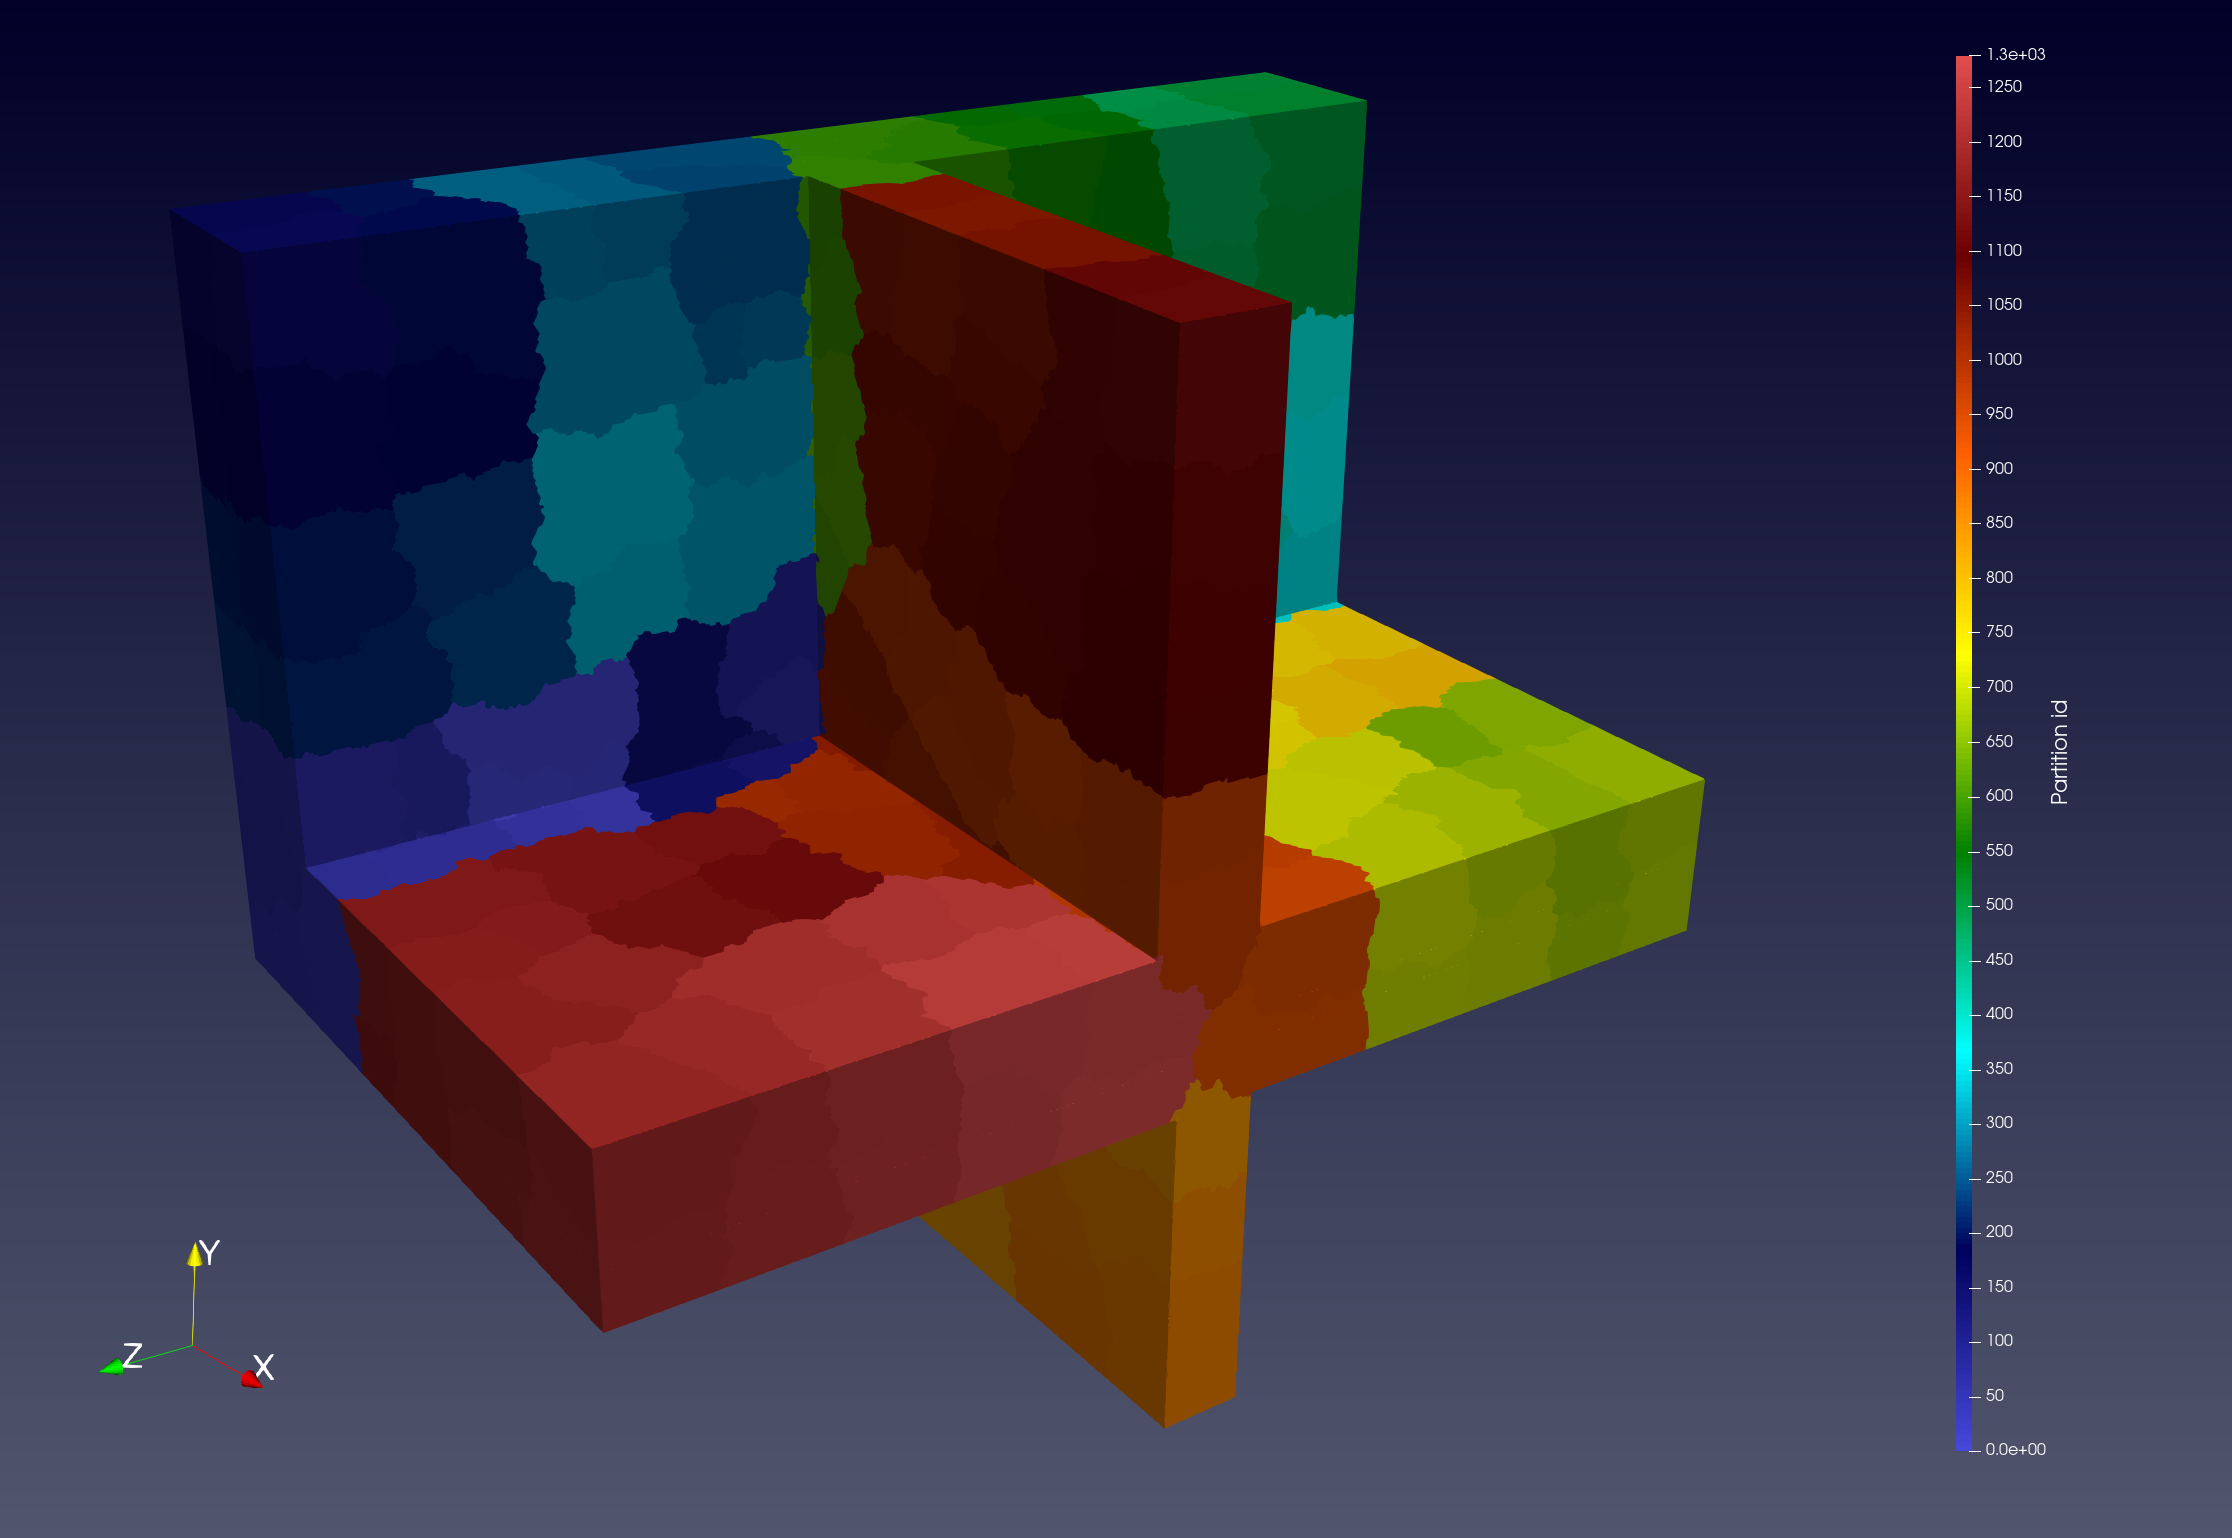
\includegraphics[width=\textwidth]{graphics/feelpp/feelpp-benchmark-thermalbridges-pid.png}
  \end{subfigure}
  \caption{Thermal bridges benchmarks - temperature solution (left) and
    partitioning example (right)}
  \label{fig:spec:app-feelpp-discr-1:thermal_bridges:visualization}
\end{figure}


\subsubsection{Mesh converging}

\todo{Insert results of mesh converging, with comparison with the reference values of the benchmark \texttt{benchmark-verification}}


\begin{figure}[ht]
  \centering
  \captionsetup[subfigure]{justification=centering}

  \pgfplotstableread[col sep=comma]{\currfiledir data.old/thermalbridges_measures.csv}\dataTableMeasures
  \def\myLineWidth{2pt}
  \def\myLineStyleA{loosely dashdotdotted} %dashdotdotted
  \def\myLineStyleB{dashed}
  \def\myLineStyleC{solid}

  \def\myAddPlot#1#2#3#4{
    \addplot[#3,every mark/.append style={solid},
    % x filter/.expression={(\thisrow{PolyOrder} == 1 ?  \pgfmathparse{\thisrow{Mesh}}\pgfmathresult :NaN)},
    % x filter/.expression={ \thisrow{FunctionSpace} == \thisrow{FunctionSpace} ? \pgfmathresult
    % x filter/.expression={(\thisrow{FunctionSpace} == P1 ? \pgfmathresult :NaN )},
      x filter/.code={
        \pgfmathparse{\thisrow{PolyOrder}==#2}
        \ifnum0=\pgfmathresult
        \pgfmathsetmacro{\newx}{nan}
      \else
        \pgfmathsetmacro{\newx}{\thisrow{Mesh}}
      \fi
      \pgfmathparse{\newx}
      },
      y filter/.expression={ #4*\pgfmathresult }
    ] table [x=Mesh, y=#1] {\dataTableMeasures};
  }

  \def\myPlotOutputMeasures#1#2#3#4{
    \resizebox{\textwidth}{0.6172\textwidth}{
      \begin{tikzpicture}
        \begin{axis}[
          width=\textwidth, height=0.6172\textwidth,
          % width=\textwidth, height=1.2\textheight,
          xtick=data,
          xticklabel={M$\pgfmathprintnumber{\tick}$},
          xmajorgrids=true,% xminorgrids=false, minor x tick num=3,
          ymajorgrids=true, yminorgrids=true,
          minor y tick num=2,
          % xticklabel={\pgfmathparse{100*\tick}\pgfmathprintnumber[precision=0]{\pgfmathresult}\%},
          % xticklabel={\pgfmathparse{\tick}\pgfmathprintnumber[fixed,set thousands separator={},precision=0]{\pgfmathresult}},
          xlabel={Mesh levels}, ylabel={#4},
          % legend style={at={(0.5,1)}, anchor=south,font=\small,legend columns=3}
          % legend style={at={(0.,1)}, anchor=north west,font=\small,legend
          % columns=3},
          legend style={at={(0.,1)}, anchor=south west,font=\small,legend columns=4},
          % #2
          ]

          \myAddPlot{#1}{1}{color=customdarkblue,\myLineStyleC,mark=o,line width=\myLineWidth}{#2}
          \addlegendentry{P1}
          \myAddPlot{#1}{2}{color=customcyan,\myLineStyleC,mark=triangle,line width=\myLineWidth}{#2}
          \addlegendentry{P2}
          \myAddPlot{#1}{3}{color=customorange,\myLineStyleC,mark=square,line width=\myLineWidth}{#2}
          \addlegendentry{P3}
          \addplot+[color=red,\myLineStyleB,mark=none,line width=\myLineWidth,every mark/.append style={solid}] coordinates {
            (1,#3) (3,#3)
          };
          \addlegendentry{Ref}

        \end{axis}
      \end{tikzpicture}
    }

  }

  \begin{subfigure}[c]{0.49\textwidth}
    \centering
    \myPlotOutputMeasures{Normal_Heat_Flux_alpha}{1}{46.09}{Heat flow [W]}
    \caption{Heat flow measured in $\alpha$ environment}
  \end{subfigure}
  \hfill
  \begin{subfigure}[c]{0.49\textwidth}
    \centering
    \myPlotOutputMeasures{Normal_Heat_Flux_beta}{1}{13.89}{Heat flow [W]}
    \caption{Heat flow measured in $\beta$ environment}
  \end{subfigure}
  \hfill
  \begin{subfigure}[c]{0.49\textwidth}
    \centering
    \vspace*{0.03\textheight}
    \myPlotOutputMeasures{Normal_Heat_Flux_gamma}{-1}{59.98}{Heat flow [W]} % warning inverse
    \caption{Heat flow measured in $\gamma$ environment}
  \end{subfigure}
  \hfill
  \begin{subfigure}[c]{0.49\textwidth}
    \centering
    \vspace*{0.03\textheight}
    \myPlotOutputMeasures{Statistics_temperature_alpha_min}{1}{11.32}{Temperature
      [°C]}
    \caption{Surface temperature min in $\alpha$ environment}
  \end{subfigure}

  \caption{Thermal bridges benchmarks - Convergence of validation measures compared to references values}
  \label{fig:spec:app-feelpp-discr-1:thermal_bridges:measures_convergences}
\end{figure}



\subsection{Times of execution}

\todo{Insert figure with time of execution of the main components described above, for the three meshes (\texttt{strong-scalability}, \texttt{weak-scalability})}


\foreach [expand list=true] \meshId in {1,2,3} {

  \pgfplotstableread[col sep=comma]{\currfiledir data.old/thermalbridges_M\meshId_P1_discoverer.csv}\dataPa
  \pgfplotstableread[col sep=comma]{\currfiledir data.old/thermalbridges_M\meshId_P2_discoverer.csv}\dataPb
  \pgfplotstableread[col sep=comma]{\currfiledir data.old/thermalbridges_M\meshId_P3_discoverer.csv}\dataPc

  \begin{figure}
    \centering
    \def\plotSetup##1{
      {table=##1,column=init,legend=Init,color=customdarkblue},
      {table=##1,legend=Assembly,column=algebraic-assembly,color=customcyan},
      %{table=##1,legend=Solve,column=algebraic-solve,color=customorange},
      {table=##1,legend=PostProcess,column=exportResults,color=customorange}
    }
    \def\chartBarPlot##1##2{
      \barChart[ybar,
      width=\textwidth, height=0.6172\textwidth,
      xticklabels from table={##2}{nProc},
      legend style={at={(0.5,1)}, anchor=south,font=\tiny,legend columns=-1}
      ]{\plotSetup{##1}}
    }
    \def\chartBarStackedPlot##1##2{
      \barChart[ybar stacked,
      width=\textwidth, height=0.6172\textwidth,
      xticklabels from table={##2}{nProc},
      legend style={at={(0.5,1)}, anchor=south,font=\tiny,legend columns=-1}
      ]{\plotSetup{##1}}
    }

    \begin{subfigure}[c]{0.49\textwidth}
      \centering
      \chartBarPlot{dataPa}{\dataPa}
      \caption{\texttt{M\meshId} - \texttt{$P_1$}}
    \end{subfigure}
    \hfill
    \begin{subfigure}[c]{0.49\textwidth}
      \centering
      \chartBarStackedPlot{dataPa}{\dataPa}
      \caption{\texttt{M\meshId} - \texttt{$P_1$}}
    \end{subfigure}
    \hfill
    \vspace*{0.04\textwidth}
    \begin{subfigure}[c]{0.49\textwidth}
      \centering
      \chartBarPlot{dataPb}{\dataPb}
      \caption{\texttt{M\meshId} - \texttt{$P_2$}}
    \end{subfigure}
    \hfill
    \begin{subfigure}[c]{0.49\textwidth}
      \centering
      \chartBarStackedPlot{dataPb}{\dataPb}
      \caption{\texttt{M\meshId} - \texttt{$P_2$}}
    \end{subfigure}
    \hfill
    \vspace*{0.04\textwidth}
    \begin{subfigure}[c]{0.49\textwidth}
      \centering
      \chartBarPlot{dataPc}{\dataPc}
      \caption{\texttt{M\meshId} - \texttt{$P_3$}}
    \end{subfigure}
    \hfill
    \begin{subfigure}[c]{0.49\textwidth}
      \centering
      \chartBarStackedPlot{dataPc}{\dataPc}
      \caption{\texttt{M\meshId} - \texttt{$P_3$}}
    \end{subfigure}
    \caption{Thermal bridges benchmarks - Execution time of main simulation components
      - Mesh \texttt{M\meshId} - Discoverer supercomputer}
    \label{fig:spec:app-feelpp-discr-1:thermal_bridges:performance_times_M\meshId}
  \end{figure}
}

\subsubsection{Scalability on IO}


\todo{Add results}
  
% \input additional app specs as needed

\section{Software Framework Contributions}

\paragraph{CGAL.} The AABB tree component of CGAL provides an efficient hierarchy of axis aligned bounding boxes that accelerates collision detection and distance queries. The hierarchy enables rapid culling of non‑candidates through AABB–AABB and query‑AABB intersection tests.  

% Traversal Strategy and Load Balancing
We integrate the AABB tree with massive parallel GPU processing to reduce geometric tests and exploit SIMD and SM execution. One query AABB is assigned per GPU thread or warp and the tree is traversed in parallel to locate intersecting leaves. Query grouping and work ordering preserve memory access coherence and mitigate divergence.  

% Traversal Strategy and Load Balancing
A stackless traversal replaces per‑thread stacks to prevent stack overuse and to enable dynamic redistribution of work across thread blocks. A shared queue dispatches nodes for exploration and permits work to be rebalanced when threads complete early. This design reduces per‑thread state and improves overall utilization of GPU resources.  

% Memory Layout and Kernel Design
AABBs and associated indices are stored contiguously and aligned to enable coalesced reads. Per‑node metadata such as child indices and primitive ranges are precomputed to minimize fetches and branch overhead. Leaves are compacted to reduce memory latency. CUDA kernels separate static hierarchy construction from real‑time query passes to confine synchronization‑heavy operations to the build phase and keep query kernels lightweight.  

% Performance Results and Limitations
The combined approach yields large reductions in pairwise detection cost, with observed speedups spanning one to three orders of magnitude relative to a naive single‑core CPU baseline depending on scene density and available parallelism. Limitations include increased memory overhead for very deep hierarchies and sensitivity to traversal divergence. Final gains are strongly dependent on partition quality and the organization of queries.  

% Future Directions
Planned improvements include adaptive query reordering to enhance load balance, hybridizing the GPU BVH with spatial grid structures for pathological or extreme distributions, and exploring probabilistic or approximate traversals for error‑tolerant applications. These directions target robustness to divergence, reduced memory footprint in deep trees, and controlled trade‑offs between accuracy and throughput.

% • FEEL++: …  
% • Mmg/ParMmg: …  

% • FEEF module: …

\section{Preliminary Benchmarks \& Trends}

% • Scaling results placeholder  




% • Energy efficiency placeholder  

% • Regression test pass-rate placeholder

\section{Roadmap \& Next Steps}

The following deliverables are planned:
\begin{itemize}
    \item D1.1-S: Software toolboxes for mesh generation and adaptation, space-time discretisation and coupling - final version planned for M60.
    \item D1.3-B: Benchmarking analysis report, including bottlenecks and breakthroughs - final version planned for M60.
\end{itemize}
Benchmarking activities are performed in interactions with WP7 and in particular T7.1.

% • Deliverables D1.x to complete by Mxx  
% • New apps to integrate into WP7 CI/CD  
% • Dependencies on WP7 infrastructure (containers, ReFrame)  